\section{Training and Development}

\subsection{TVS}
TVS Motor Company places a strong emphasis on the training and development of its employees, recognizing that a skilled and knowledgeable workforce is essential for driving innovation and maintaining competitive advantage in the automotive industry. The company employs a multi-faceted approach to employee development, offering a variety of training programs designed to enhance technical skills, leadership capabilities, and overall professional growth. Through initiatives such as the TVS Institute of Quality \& Leadership (IQL), employees benefit from tailored learning experiences, continuous education, and opportunities for skill-building in emerging technologies, including electric vehicles, software, data analytics, and artificial intelligence.

Additionally, TVS Motor fosters a culture of continuous improvement by encouraging employees to participate in global partnerships, professional development programs, and innovative learning solutions, such as virtual reality (VR) and augmented reality (AR) training. This comprehensive training and development framework not only equips employees with the necessary competencies to excel in their roles but also aligns with TVS Motor's strategic objectives of driving excellence and sustainability in its operations.

They follow a set of principles\cite{tvsmotorMotorCompany}\cite{tvsmotorMotorCompanyMission}. They are:

\textbf{P1:} businesses should conduct and govern themselves with integrity, and in a manner that is ethical, transparent and accountable. \\\textbf{P2:} businesses should provide goods and services in a manner that is sustainable and safe. \\\textbf{P3:} businesses should respect and promote the well-being of all employees, including those in their value chains.

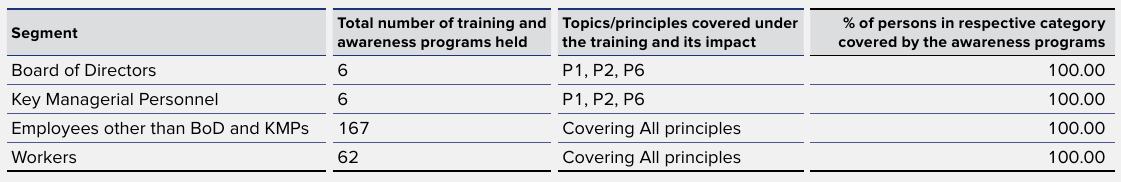
\includegraphics[width=\linewidth]{psycho_images/TVS_Training.png}

\subsection{Hero}

\textbf{Technical Training}\\
The company offers specialized technical training programs that cover essential areas such as CNC programming, auto-gauging, hydraulics, pneumatics, and electrical drives. Additionally, employees receive training in Integrated Management System (IMS) awareness, Total Productive Maintenance (TPM), and the Jishu Hozen (JH) and Kobetsu Kaizen (KK) pillars. These programs are designed to equip employees with the necessary technical expertise to excel in their roles across various segments of the workforce.

\textbf{Behavioral Training}\\
Hero MotoCorp also invests in behavioral training initiatives aimed at enhancing soft skills among its employees. These programs focus on nurturing workplace relationships, promoting assertive communication, and instilling the company's core values. Furthermore, sensitization programs covering topics such as the Prevention of Sexual Harassment (POSH), gender sensitization, unconscious bias, and adherence to the Code of Conduct are integral to fostering a respectful and inclusive workplace culture.

\textbf{Functional Programs}\\
In line with its commitment to continuous improvement, Hero MotoCorp provides functional training programs that enable employees to upskill their data analytical capabilities. This includes training in critical areas such as the 7 Quality Control (QC) tools, Advanced Excel, and Power BI, empowering the workforce to leverage data effectively for decision-making and operational excellence.

These initiatives reflect Hero MotoCorp's dedication to fostering a skilled, knowledgeable, and inclusive workforce that can adapt to the evolving demands of the industry.

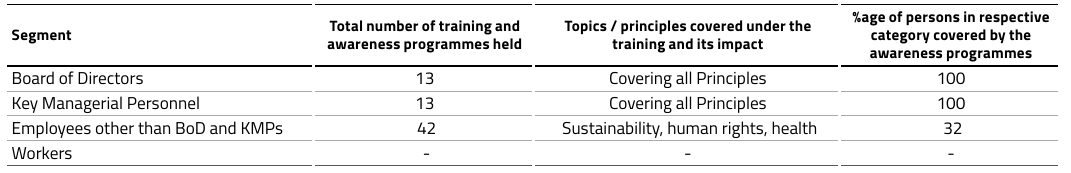
\includegraphics[width=\linewidth]{psycho_images/Hero_Training.png}

Here is a summary of the overall training hours and money invested:

\textbf{Total training hours}: 11,18,505 \\
\textbf{Average training hours / employee}: 32.93 \\
\textbf{Average spent on training and development per employee} (includes staff and permanent workers): Rs 10,488 \\

